\documentclass[11pt]{article}
\usepackage[spanish]{babel}


%%%%%%%%%%%%%%%%%%%%%%%%%%%%%%%%%%
%%%%%%%%%%%%%%%%%%%%%%%%%%%%%   %%
%%        Datos Trabajo     %%  %%
%%%%%%%%%%%%%%%%%%%%%%%%%%%%%%%%%%
\newcommand{\titulo}[0]{Reto 2. Casos de estudio}
\newcommand{\materia}[0]{Finanzas Personales v1}


%%%%%%%%%%%%%%%%%%%%%%%%%%%%%%%%%%
%%%%%%%%%%%%%%%%%%%%%%%%%%%%%%%%%%
\usepackage{amssymb}
\usepackage{enumerate}
\usepackage{geometry}
\usepackage{mathtools}
\usepackage{multicol}
\usepackage{soul}

\usepackage{graphicx}
	\graphicspath{ {assets/} }

\usepackage{hyperref}
	\hypersetup{
			pdftex,
		        pdfauthor={bench},
		        pdftitle={...},
		        pdfsubject={...},
		        pdfkeywords={UVEG},
		        pdfproducer={Latex with hyperref, Ubuntu},
		        pdfcreator={pdflatex, or other tool},
			colorlinks=true,
				linkcolor=[rgb]{0,0,0.45},
				urlcolor=cyan,
				filecolor=green,
				citecolor=blue}

%%%%%%%%%%%%%%%%%%%%%%%%%%%%%%%%%%
%%%%%%%%%%%%%%%%%%%%%%%%%%%%%%%%%%

\title{\titulo}

\author{ Universidad Virtual del Estado de Guanajuato \textbf{UVEG} \\ 
\materia \\ Benjamín Rivera \\ 19015478 }
\date{\textit{Fecha de entrega:} \today}


%%%%%%%%%%%%%%%%%%%%%%%%%%%%%
%%        Documento         %%
%%%%%%%%%%%%%%%%%%%%%%%%%%%%%%%
\begin{document}
	\maketitle
	
	\begin{figure}[htp]
		\centering
		
\includegraphics[width=\textwidth]{assets/R2_U1-plan_allianz.png}
		\caption{Características del plan que propone allianz obtenido de \cite{plan}}
		\label{plan}
	\end{figure}
	
	\par Hay dos razones principales por las cuales considero que este es uno de los mejores planes de ahorro para este objetivo
	
	\begin{enumerate}
		\item La opción de \textbf{ Periodo de descanso } permitiría no estar completamente amarrado a este, dando flexibilidad para algún percance o emergencia que pudiera surgir con el tiempo; y
		\item la confianza y buen servicio que la empreza \textbf{ Allianz } le a dado a mi familia con el tiempo.
	\end{enumerate}
	
	\noindent En complemento a las dos razones anteriores, este plan ofrece prestaciones esenciales para un ahorro educativo.
	\\\ \\
	\par Para este ejercicio se considera que se cubrirán colegiaturas y manutención durante 5 años. Supondremos los precios para el primer año y luego solo los inflaremos a una taza promedio de $4\%$. Además no contamos con nada ahorrado por el momento.
	
	\begin{quote}
	\begin{description}
		\item [Colegiatura] Se apoyara para una colegiatura anual de \textbf{ \$25,000 }
		\item [Manutención] Se apoyara para una manutención anual de \textbf{ \$38,000 }
		\item [Monto total] De manera que (considerando la inflación anual) en total se necesitan \textit{ aproximadamente } \textbf{ \$341,228.32}. Lo cual seria bueno redondear a \textbf{ \$350,000.00} para poder cubrir cualquier eventualidad.
		\item [Plazo] Dado que empiezo cuando mi hijo acaba de cumplir 5 años, \textbf{tengo 13 años} antes de que vaya a la universidad.
	\end{description}
	\end{quote}
	
	\begin{figure}[htp]
		\centering
		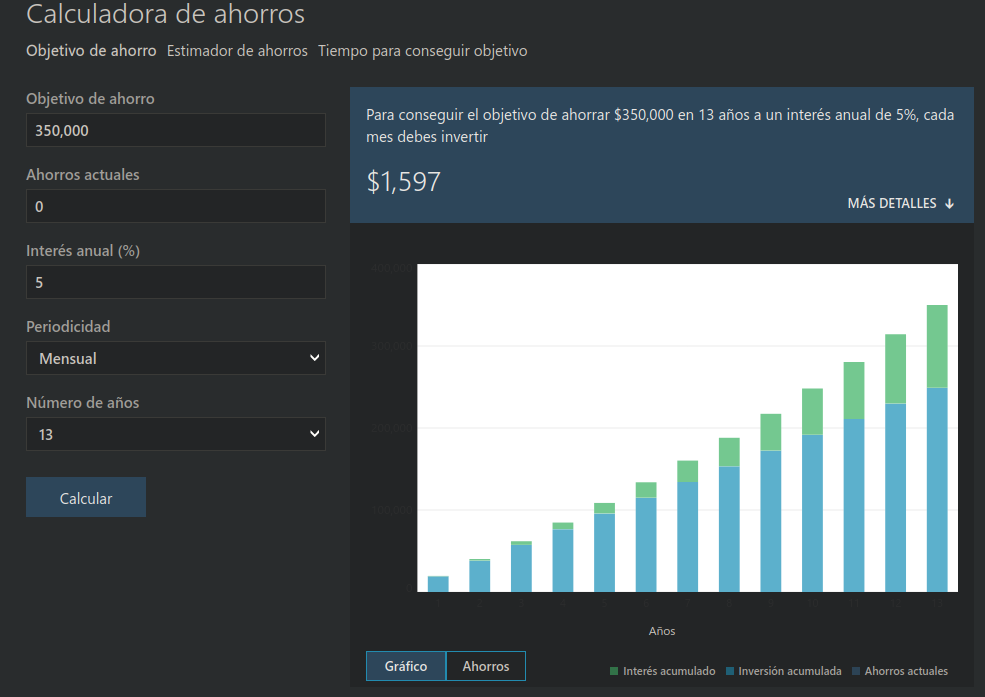
\includegraphics[width=0.8\textwidth]{assets/R2_U1-calc_ahorro.png}
		\caption{Plan de ahorro con los datos obtenidos de \cite{calc 1}.}
		\label{}
	\end{figure}

\section{Conclusi\'on}
	
	\par Esta me ha parecido una maravillosa primera actividad, de manera simple y concisa, además de que con un ejemplo bastante real (que por desgracia) la mayoría de nosotros deberemos afrontar al menos una vez en nuestras vidas. En conclusión, después de hacer esta actividad, he notado dos cosas muy importantes. 
	\par La primera, que mientras empiece con tiempo, lograr metas financieras como esta (que se pueden considerar grandes) no requiere de esfuerzos demasiado grandes. Y se reduce aún más el impacto cuando se tiene la ventaja de que se divide la responsabilidad con tu pareja e incluso (cuando se tiee mucha suerte) con más miembros de la familia (como tios, abuelos, entre otros).
	\par La segunda, que la perseverancia y la disciplina son herramientas esenciales para poder gozar de una buena salud financiera. Y que a pesar de que hay cosas que se escapan al poder de estas dos virtudes, el alcance de metas objetivas si están en su abanico de posibilidades siempre que se empiece con tiempo; dado que esto permite poder escoger un buen plan y aprovecharse del interés compuesto a su favor (para variar y no solo pagarlo cuando nos atrasamos con créditos).
	\\\
	\par De manera general podemos ver que con la planeación correcta, la disciplina para ahorrar constantemente, el conocimiento y la paciencia para encontrar el producto financiero que mejor se adapte a nuestras necesidades y con el tiempo adecuado, las metas financieras y, por lo tanto, nuestra salud financiera, es algo que perfectamente podemos cuidar y mantener en buenos niveles de salúd.



%%%%%%%%%%%%%%%%%%%%%%%%%%%%%%%%
%%         Bibliografia        %%
%%%%%%%%%%%%%%%%%%%%%%%%%%%%%%%%%%

	\begin{thebibliography}{X}
	
		\bibitem{plan} Ahorro para la educación. (s/f). Allianz Mexico. Recuperado el 20 de enero de 2021, de \url{https://www.allianz.com.mx/seguros/ahorro-e-inversion/seguro-educacion.html}

		\bibitem{calc 1} Calculadora de ahorros—MSN Dinero. (s/f). MSN. Recuperado el 20 de enero de 2021, de \url{https://www.msn.com/es-mx/dinero/herramientas/calculadora-de-ahorros}

		\bibitem{calc 2} Suncoast Credit Union. (s/f). Recuperado el 20 de enero de 2021, de \url{https://es.suncoastcreditunion.com/resources/calculators/college-savings-calculator-es}

	
	\end{thebibliography}

\end{document}